%\documentclass[12pt,serif]{beamer}
%\documentclass[tikz,12pt,svgnames]{beamer}
\documentclass[table,handout,tikz,12pt,svgnames]{beamer}
\usepackage{CM-preamble}
\subtitle{\Huge Structures cartésiennes}
%\date{1 février 2016}
%\date{29 janvier 2016}
\date{CM1}

\begin{document}

\begin{frame}
	\titlepage
\end{frame}

%\begin{frame}
%  \frametitle{Outline}
%  \tableofcontents
%\end{frame}

\begin{frame}[fragile=singleslide]
	\frametitle{Tableaux}
	\begin{itemize}
%		\begin{block}{Tableaux}
		\vspace{-1cm}
		\begin{block}{}			
			\item Collections indicées d'informations de même type (homogène)
		\end{block}
		
		\begin{tikzpicture}[font=\ttfamily,
		array/.style={matrix of nodes,nodes={draw, minimum size=7mm, fill=green!60},column sep=-\pgflinewidth, row sep=0.5mm, nodes in empty cells,
			row 1/.style={nodes={draw=none, fill=none, minimum size=5mm}},
			row 1 column 1/.style={nodes={draw}}}]
		
		\matrix[array] (array) {
			0 & 1 & 2 & 3 & 4 & 5 & 6 & 7 & 8 & 9\\
			&   &   &   &   &   &   &   &   &  \\};
		\node[draw, fill=orange, minimum size=4mm] at (array-2-9) (box) {};
		
		\begin{scope}[on background layer]
		\fill[gray!25] (array-1-1.north west) rectangle (array-1-10.south east);
		\end{scope}
		
		\draw[<->]([yshift=-3mm]array-2-1.south west) -- node[below] {Tableau de longeur 10} ([yshift=-3mm]array-2-10.south east);
		
		\draw (array-1-1.north)--++(90:3mm) node [above] (first) {Premier indice};
		\draw (array-1-10.east)--++(0:3mm) node [right]{Indices};
		\node [align=center, anchor=south] at (array-2-9.north west|-first.south) (8) {Élement\\ (à l'indice 8)};
		\draw (8)--(box);
		%
		\end{tikzpicture}
		
		
	\end{itemize}
	\begin{itemize}
		\begin{block}{Types de données}
			\item char, short, int, long, long long, float, double, long double
		\end{block}
	\end{itemize}
\end{frame}	
	
\begin{frame}[fragile=singleslide]
	\frametitle{Structures cartésiennes}
	\begin{itemize}
%		\begin{block}{Structures}
		\vspace{-2cm}
		\begin{block}{}
			\item n-uplet d'informations de types quelconque rangées dans des champs
			\begin{itemize}
				\item Informations complexes (composites)
				\item Des « types de variables personnalisés »
			\end{itemize}

			\item Notation
			\begin{minted}[
			mathescape=true,
			escapeinside=||,			
		%	frame=lines,
		%	framesep=1.5mm,
		%		baselinestretch=0.4,
		%		fontsize=\footnotesize,
		%		linenos
		]{c}
	|\underline{type}| <ST> = |\underline{structure}|
		champ1: <T1>
		champ2: <T2>
		...
		champn: <Tn>
	|\underline{fin}|		
			\end{minted}
		\end{block}
	\end{itemize}
\end{frame}


\begin{frame}[fragile=singleslide]
	\frametitle{Structures cartésiennes}
	\begin{itemize}
		%		\begin{block}{Structures}
%		\vspace{-2cm}
		\begin{block}{Domaine des valeurs d'une structure}
			\item Produit cartésien des domaines des champs
			\begin{itemize}
				\item $Dom(ST)=Dom(T_1) \bigtimes Dom(T_2) \bigtimes \ldots \bigtimes Dom(T_n)$
			\end{itemize}
			\item Accès aux champs par notation pointée
			\begin{itemize}
				\item $v:<ST>$, accès au champs i  $v.champ_i$
			\end{itemize}
		\end{block}
		\begin{block}{Example}
			\begin{minted}[
			mathescape=true,
			escapeinside=||,
			]{text}
	|\underline{type}| Ouvrage = |\underline{structure}|
		code: Entier
		titre: Chaine
	|\underline{fin}|
			\end{minted}
		\end{block}
	\end{itemize}
\end{frame}

\begin{frame}[fragile=singleslide]
	\frametitle{Structures cartésiennes}
	\begin{minted}[mathescape=true,escapeinside=||]{text}
|\underline{type}| Complexe = |\underline{structure}|
	reelle, imag: Reel
|\underline{fin}|
	\end{minted}
	\vspace{-0.9cm} \myline  \vspace{-0.7cm}	
	\begin{minted}[mathescape=true,escapeinside=||,
%		frame=lines,
%		framesep=2mm,
	]{text}
|\underline{fonction}| plus(c1,c2) : Complexe
	|\underline{donnees}|: c1,c2: Complexe
	|\underline{locales}|: c: Complexe
	c.reelle := c1.reelle + c2.reelle
	c.imag := c1.imag + c2.imag
	résultat: c
|\underline{finfonction}|
	\end{minted}			
	\vspace{-0.9cm} \myline  \vspace{-0.5cm}	
Utilisation:	
	\begin{minted}[mathescape=true,escapeinside=||]{text}

c1,c2,c3 : Complexe
c3 := plus(c1,c2)
	\end{minted}			
\end{frame}


\begin{frame}[fragile=singleslide]
	\frametitle{Structures imbriquées}
	\begin{itemize}
		%		\begin{block}{Structures}
		\vspace{-0.9cm}
		\begin{block}{}
			\item Le types des champs est quelconque
			\begin{itemize}
				\item Ils peuvent même être des structures
			\end{itemize}
			\begin{minted}[
			mathescape=true,
			escapeinside=||,			
			]{c}
|\underline{type}| Date = |\underline{structure}|
	jour, mois, annee : Entier
|\underline{fin}|		
			\end{minted}
			\begin{minted}[
			mathescape=true,
			escapeinside=||,			
			]{c}
|\underline{type}| Fiche = |\underline{structure}|
	emprunt : Ouvrage
	date : Date
|\underline{fin}|
			\end{minted}
		\end{block}
	\end{itemize}
	\vspace{-1.1cm} \myline  \vspace{-1.4cm}
	\begin{block}{}
		\begin{minted}[mathescape=true,	escapeinside=||,]{c}
//F est une variable de type Fiche
F: Fiche 
  //Les accès aux champs sont de type
  |$\Rightarrow$| F.date: Date |$\Rightarrow$| F.date.jour: Entier
  |$\Rightarrow$| F.emprunt: Ouvrage |$\Rightarrow$| F.emprunt.titre: Chaine
		\end{minted}
	\end{block}		
\end{frame}


\begin{frame}[fragile=singleslide]
	\frametitle{Tableaux de structures}
		%		\begin{block}{Structures}
%		\vspace{-0.2cm}
%	\begin{block}{}%Exemple Emprunts and semaine:7 jours, jours féries}
%		\begin{figure}
%			\resizebox{\linewidth}{!}{%
	  \begin{columns}[onlytextwidth]
	  	\begin{column}{0.5\textwidth}
			\texttt{locations}\\
			\centering
			\begin{tikzpicture}[font=\ttfamily]
				\foreach \index/\list in {0/{ficheA}, 1/{ficheC}, 2/{ficheZ}} {
					\node[array element] (aux) at (0,-\index*0.8) {\index};
					\ArrayList{\list}
				}
			\end{tikzpicture}\\
			\ldots\\
			%END NODE
			\begin{tikzpicture}[font=\ttfamily]
						\foreach \index/\list in {0/{ficheX}} {
							\node[array element] (aux) at (0,-\index*0.8) {n-1};
							\ArrayList{\list}
						}
			\end{tikzpicture}\\
		\end{column}
		\begin{column}{0.5\textwidth}
		    	\texttt{j\_feries}\\
		    	\centering
		    		\begin{tikzpicture}[font=\ttfamily]
		    			\foreach \index/\list in {0/{date11}, 1/{date22}, 2/{date14}, 3/{date22}, 4/{date22}} {
		    				\node[array element] (aux) at (0,-\index*0.8) {\index};
	    					\ArrayList{\list}
	    				}
    				\end{tikzpicture}\\
		    				
		       \end{column}
		\end{columns}
%			}		
%		\end{figure}
%	\end{block}
	\vspace{-0.2cm} \myline \vspace{-1.2cm}
	\begin{block}{}
		\begin{minted}[mathescape=true,	escapeinside=||,]{c}
//Accès
locations : vecteur[N] de Fiche
f: Fiche ; f |$\leftarrow$| locations[3]
    |$\Rightarrow$| f.date: Date |$\Rightarrow$| f.date.jour: Entier
    |$\Rightarrow$| f.emprunt: Ouvrage |$\Rightarrow$| f.emprunt.titre: Chaine
		\end{minted}
	\end{block}		
\end{frame}


\begin{frame}[fragile=singleslide]
	\frametitle{Déclaration de structures en C}
	\begin{itemize}
		%		\begin{block}{Structures}
%		\vspace{-2cm}
		\begin{block}{}
			\item Le mot clé \texttt{struct} permet de définir des modèles de structures:
			\begin{minted}[
			mathescape=true,
			escapeinside=||,			
			%	frame=lines,
			%	framesep=1.5mm,
			%		baselinestretch=0.4,
			%		fontsize=\footnotesize,
			%		linenos
			]{c}
    struct <désignateur> {
	    <déclaration de champ1>;
	    <déclaration de champ2>;
	    |$\ldots$|
	    <déclaration de champn>;
    }; //Point-virgule obligatoire
	   		\end{minted}
		\end{block}
		où:
		\item \texttt{<désignateur>} est le nom (facultatif) du modèle
		\item \texttt{<declarations de champ>} comme des déclarations de var mais sans initialisation
	\end{itemize}
\end{frame}


\begin{frame}[fragile=singleslide]
	\frametitle{Exemples de structures en C}
	\begin{minted}[
			mathescape=true,
			escapeinside=||,			
			%	frame=lines,
			%	framesep=1.5mm,
			%		baselinestretch=0.4,
			%		fontsize=\footnotesize,
			%		linenos
			]{c} 
/* definition de la structure*/
struct date {int j,m,a;}; 

/*2 variables selon le modèle date*/
struct date d1, d2;

/*definition et utilisation immédiate*/
struct complexe {float reelle, imag;} c1, c2;

/*rappel du même modèle*/
struct complexe c3;
	\end{minted}
\end{frame}

%TODO: FIGURE OUT WHAT THIS SLIDE WAS SUPPOSED TO BE
%\begin{frame}[fragile=singleslide]
%	\frametitle{Exemples de structures en C}
%	\vspace{0.0cm}
%		\inputminted[
%%		frame=lines,
%%		framesep=2.5mm,
%		baselinestretch=0.65,
%		fontsize=\footnotesize,
%		linenos,
%		tabsize=4,
%%		bgcolor=light-gray
%		]
%		{c}{../codes/struct_example.c}
%\end{frame}

\begin{frame}[fragile=singleslide]
	\frametitle{Définitions de synonymes de types (typedef)}
	\begin{itemize}
		%		\begin{block}{Structures}
		\vspace{-0.5cm}
		\begin{block}{}
			\item \texttt{typedef} permet de donner des alias (synonymes) à des définitions de types dans toute zone déclarative :
			\begin{minted}[
			mathescape=true,
			escapeinside=||,			
			%	frame=lines,
			%	framesep=1.5mm,
			%		baselinestretch=0.4,
			%		fontsize=\footnotesize,
			%		linenos
			]{c} 
typedef <un_type> <synonyme_du_type>
			\end{minted}
			\texttt{<un\_type>} a la même syntaxe qu'une déclaration de variable, et  \texttt{<synonyme\_du\_type>} désigne le nouveau nom du type
		\end{block}
		\vspace{-0.3cm}
		\begin{block}{}
			\item Donne des noms plus simples pour faciliter l'écriture et augmenter la lisibilité 
		\end{block}
		\begin{block}{}
			\item Examples :
			\begin{minted}[
			mathescape=true,
			escapeinside=||,			
			%	frame=lines,
			%	framesep=1.5mm,
			%		baselinestretch=0.4,
			%		fontsize=\footnotesize,
			%		linenos
			]{c} 
typedef unsigned char octet;
typedef struct ma_structure * ma_struct;
typedef struct S S;
			\end{minted}				
		\end{block}
	\end{itemize}
\end{frame}


\begin{frame}[fragile=singleslide]
	\frametitle{Tableaux de structures}
		\vspace{-0.2cm}
%	\begin{block}{}%Exemple Emprunts and semaine:7 jours, jours féries}
%		\begin{figure}
%			\resizebox{\linewidth}{!}{%
	  \begin{columns}
	  	\begin{column}{0.45\textwidth}
		  	Exemples :
			\begin{minted}[mathescape=true,	escapeinside=||,fontsize=\footnotesize,,baselinestretch=1.2]{c}
typedef int * PtInt;
typedef int Matrice[10][20];
typedef struct date Date;
typedef struct {
    int numero;
    char titre[50];
} Ouvrage;
			\end{minted}
		\end{column}
%		\setlength{\columnseprule}{0.4pt}
		\vrule{}
		\begin{column}{0.55\textwidth}
			Conséquences
			\begin{minted}[mathescape=true,	escapeinside=||,fontsize=\footnotesize,baselinestretch=1.2]{c}
PtInt p; |$\Leftrightarrow$| int * p;
Matrice m; |$\Leftrightarrow$| int m[10][20];
Date d; |$\Leftrightarrow$| struct date d;
Ouvrage o; |$\Leftrightarrow$| struct {
                  int numero;
                  char titre[50];
               } o;
			\end{minted}
	    \end{column}
	\end{columns}
	\vspace{1cm}
	Typedef rend superflu le nom du modèle (sauf dans le cas de structures récursives...).
	
%	\vspace{-0.2cm} \myline \vspace{-1.2cm}
%	\begin{block}{}
%		\begin{minted}[mathescape=true,	escapeinside=||,]{c}
%//Accés
%locations : vecteur[N] de Fiche
%f: Fiche ; f |$\leftarrow$| locations[3]
%    |$\Rightarrow$| f.date: Date |$\Rightarrow$| f.date.jour: Entier
%    |$\Rightarrow$| f.emprunt: Ouvrage |$\Rightarrow$| f.emprunt.titre: Chaine
%		\end{minted}
%	\end{block}		
\end{frame}

\begin{frame}[fragile=singleslide]
	\frametitle{Manipulations de structures: Exemple Date}
	\begin{adjustwidth}{-1.6em}{-1.5em}
		\begin{minted}[
			mathescape=true,
			escapeinside=||,			
			%	frame=lines,
			%	framesep=1.5mm,
			%		baselinestretch=0.4,
					fontsize=\footnotesize,
			%		linenos
			]{c}
typedef struct Date {int jour, mois, annee;} Date; /* option 1 */ 
typedef struct {int jour, mois, annee;} Date;      /* option 2 */ 
Date d1 = {18,5,2012} ; Date d2 = {24,12,2015};   /* variables */
sizeof(Date); /* taille de la structure Date = 3*sizeof(int) */ 
		\end{minted}
	\end{adjustwidth}
	\vspace{0.5cm}
	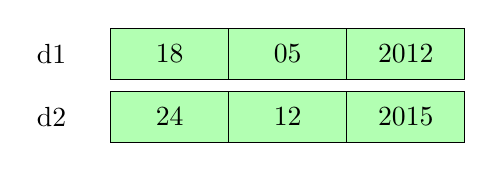
\begin{tikzpicture}
	% size of each node
	\def\sz{6.5mm}
	\def\szwidth{15mm}
	\def\offset{0.8}
	% node style definition
	\tikzstyle{block} = [draw, fill=green!30, rectangle, minimum height=\sz, minimum width=\sz ];
	\tikzstyle{rect} = [draw, fill=green!30, rectangle, minimum height=\sz, minimum width=\szwidth ];	
	\tikzstyle{plain} = [draw=none,fill=none];
	% array element definition
	\def\dateone{24,12,2015};
	\def\datetwo{18,05,2012};
	%\def\x{0}; % x pos of arr
	%\def\y{0}; % y pos of arr
	\newcounter{ind}; \setcounter{ind}{0};
	\node[plain] { d2 };
	\foreach \item in \dateone {
		\addtocounter{ind}{1};
%		\node[block] at (\theind*\sz,0) { \item };
%		\node[rect] at (\theind*\szwidth,1.7) { \item };
		\node[rect] at (\theind*\szwidth,0) { \item };
	}
	\setcounter{ind}{0};
	\node[plain] at (0,\offset) { d1 };
	\foreach \item in \datetwo {
		\addtocounter{ind}{1};
		\node[rect] at (\theind*\szwidth,\offset) { \item };
	}
	\end{tikzpicture}

	\vspace{-0.3cm}
	\begin{itemize}
		\begin{block}{}
			\item Sélection de champ : opérateur \texttt{\textbf{.}} de plus forte priorité
			\begin{minted}[
			mathescape=true,
			escapeinside=||,			
			%	frame=lines,
			%	framesep=1.5mm,
			%		baselinestretch=0.4,
			%		fontsize=\footnotesize,
			%		linenos
			]{c} 
d1.jour = d2.jour;
scanf("%d",&d2.jour);
/* équivalent à scanf("%d", &(d2.jour)); */
			\end{minted}				
		\end{block}
	\end{itemize}
\end{frame}


\begin{frame}[fragile=singleslide]
	\frametitle{Affectation entre structures}
	\begin{itemize}
		%		\begin{block}{Structures}
		\vspace{-0.7cm}
		\begin{block}{}
			\item Copie \textbf{champs par champ} (contrairement aux tableaux).
			\begin{itemize}
				\item Attention aux pointeurs, \textbf{"shallow copy"}
			\end{itemize}
			\vspace{0.2cm}
	  \begin{columns}[T]
	  	\begin{column}{0.50\textwidth}
		  	\underline{Avec tableau}
			\begin{minted}[mathescape=true,	escapeinside=||,fontsize=\footnotesize,,baselinestretch=1.2]{c}
struct Sarray {
	int p[3];
};
struct Sarray sa1, sa2;

sa1.p[0]=10; sa1.p[1]=20;
sa1.p[2]=30;

sa2 = sa1;
			\end{minted}
		\end{column}
%		\vrule{}
		\begin{column}{0.55\textwidth}
			\underline{Avec pointeur}
			\begin{minted}[mathescape=true,	escapeinside=||,fontsize=\footnotesize,baselinestretch=1.2,linenos]{c}
struct Spointer {
	int * p;
};
struct Spointer sp1, sp2;
sp1.p = malloc(3*sizeof(*sp1.p));
sp1.p[0] = 10; sp1.p[1] = 20;
sp1.p[2] = 30;

sp2 = sp1;
free(sp1.p);
			\end{minted}
	    \end{column}
	\end{columns}
	\vspace{1cm}
		\end{block}
		\vspace{-1cm}
		
		\begin{block}{Quelles sont les différences ?}
		\end{block}
	\end{itemize}
\end{frame}

\begin{frame}
	\frametitle{Quelques limites}
	\begin{itemize}
		\begin{block}{}%Mais...}
			\item Pas de comparaisons (==, !=, >, <, ...)
			\item Pas d'opérateurs arithmétiques
			\item Pas de E/S (scanf, printf, ...) 
			\item Pas de support de "deep copy" (pas de copie des valeurs "pointées", seulement les valeurs des pointeurs)
			\item Attention aux passage des structures dans des fonctions (passage-par-copie des structs, implique "Shallow Copy")
		\end{block}
		\vspace{1cm}
		\begin{block}{\Large Beacoup de choses à programmer\\ \textit{à la main} !!!}
		\end{block}		
	\end{itemize}
\end{frame}

%		\begin{block}{Mais...}
%			\item Pas de comparaisons (==, !=, >, <, ...)
%			\item Pas de E/S (scanf, printf, ...) 
%		\end{block}
%	\end{itemize}




\begin{frame}[fragile=singleslide]
	\frametitle{Tableaux dans les structures}

%	\begin{adjustwidth}{-1.6em}{-1.5em}
%	Rappel :
		\begin{minted}[
			mathescape=true,
			escapeinside=||,			
			%	frame=lines,
			%	framesep=1.5mm,
			%		baselinestretch=0.4,
%					fontsize=\footnotesize,
			%		linenos
			]{c}
typedef struct {
	int numero;
	char titre[50];
	} Ouvrage;
Ouvrage x,y; //variables
		\end{minted}
%	\end{adjustwidth}
	\vspace{0.5cm}
	\begin{tikzpicture}
	% size of each node
	\def\sz{6.5mm}
	\def\szwidth{17mm}
	\def\offset{0.6}
	% node style definition
	\tikzstyle{block} = [draw, fill=green!30, rectangle, minimum height=\sz, minimum width=\sz ];
	\tikzstyle{rect} = [draw, fill=green!30, rectangle, minimum height=\sz, minimum width=\szwidth ];
	\tikzstyle{indices} = [rectangle, minimum height=\sz, minimum width=\szwidth ];
	\tikzstyle{plain} = [draw=none,fill=none];
	% array element definition
	\def\dateone{int,char,char,\ldots,\ldots,char};
	\def\datetwo{numéro,titre[o],titre[1],\ldots,\ldots,titre[49]};
	%\def\x{0}; % x pos of arr
	%\def\y{0}; % y pos of arr
	%\newcounter{ind};
	\setcounter{ind}{0};
	\node[plain] { x };
	\foreach \item in \dateone {
		\addtocounter{ind}{1};
%		\node[block] at (\theind*\sz,0) { \item };
%		\node[rect] at (\theind*\szwidth,1.7) { \item };
		\node[rect] at (\theind*\szwidth,0) { \item };
	}
	\setcounter{ind}{0};
	%\node[plain] at (0,\offset) { d1 };
	\foreach \item in \datetwo {
		\addtocounter{ind}{1};
		\node[indices] at (\theind*\szwidth,\offset) { \item };
	}
	\end{tikzpicture}
	\vspace{-1cm}
	\begin{itemize}
		\begin{block}{}
			\item \texttt{y = x       } {
\includegraphics[scale=0.40]{../common-images/check.pdf}}		
			\item \texttt{y.titre = x.titre    } {
\includegraphics[scale=0.40]{../common-images/attention.pdf}} \BAD{IMPOSSIBLE} 
%			\begin{itemize}
%				\item Ce n'est pas possible de copier un tableau de cette façon
%				\item Utilisez les fonctions de C dédiés : \texttt{strcpy, strncpy, strncat, \ldots}
%			\end{itemize}
		\end{block}
	\end{itemize}
	\begin{block}{Et si \texttt{titre} était un \texttt{char *} ???} \end{block}
\end{frame}


\begin{frame}[fragile=singleslide]
	\frametitle{Tableaux dans les structures}
	\begin{itemize}
		\begin{block}{}
			\item \texttt{y.titre = x.titre    } {
\includegraphics[scale=0.40]{../common-images/attention.pdf}} \BAD{IMPOSSIBLE} 
			\begin{itemize}
				\item Copiez les caractères un par un
				\item Ou utilisez les fonctions de C dédiés : \texttt{strcpy, strncpy, strncat, \ldots}
			\end{itemize}
			\vspace{0.5cm}
			\begin{adjustwidth}{-1.6em}{-1.5em}
				\begin{minted}[
			mathescape=true,
			escapeinside=||,			
			%	frame=lines,
			%	framesep=1.5mm,
			%		baselinestretch=0.4,
%					fontsize=\footnotesize,
			%		linenos
			]{c}
//attention aux caractères de fin de chaine '\0'
strcpy(y.titre, x.titre);

strncpy(y.titre, x.titre, 50); //donnez la taille
y.titre[50 - 1] = '\0';   //garantir fin de chaine

/* Ou concatener avec une chaine vide: */
*y.titre = '\0'; strncat(y.titre, x.titre, 50-1);
				\end{minted}				
			\end{adjustwidth}
		\end{block}
	\end{itemize}
\end{frame}

%ERROR from Nathalie Devesa Slides
%char * is not the same as char []
\begin{frame}[fragile=singleslide]
	\frametitle{Structures dans les structures}
			\begin{adjustwidth}{-1.6em}{-1.5em}
				\begin{minted}[
			mathescape=true,
			escapeinside=||,			
			%	frame=lines,
			%	framesep=1.5mm,
			%		baselinestretch=0.4,
%					fontsize=\footnotesize,
			%		linenos
			]{c}
typedef struct {int numero; char titre[50];} Ouvrage;
typedef struct {int jour, mois, annee;} Date;
typedef struct Fiche {
	Ouvrage emprunt ; //struct imbriquée
	Date date ;       //struct imbriquée
} Fiche ;

//Déclaration et Initialization en 1:
Fiche f = {{23,"H. Potter"}, {12,5,2006}}; //C99
				\end{minted}				
			\end{adjustwidth}
	\begin{itemize}
		\begin{block}{Accès aux champs}
			\item \texttt{f.date.jour} de type \texttt{int}
			\item \texttt{f.emprunt.titre} de type \texttt{char []}
		\end{block}
	\end{itemize}
\end{frame}

\begin{frame}[fragile=singleslide]
	\frametitle{Tableaux de structures}
	\vspace{-0.7cm}
	\begin{itemize}
		\begin{block}{}
			\item Utilisation similaire aux tableaux "normaux"
%			\item \texttt{f.emprunt.titre} de type \texttt{char []}
		\end{block}
%	\vspace{.3cm}
	\end{itemize}
			\begin{adjustwidth}{0em}{-1.5em}
				\begin{minted}[
			mathescape=true,
			escapeinside=||,			
			%	frame=lines,
			%	framesep=1.5mm,
			%		baselinestretch=0.4,
					fontsize=\footnotesize,
					linenos
			]{c}
Fiche tableau_fiches[3];
Ouvrage o1; Date d1;
//Fiche 1 : initialization des sous structures
o1.numero=23; strcpy(o1.titre,"H. Potter");
d1.jour=12 ; d1.mois=5; d1.annee=2006;
tableau_fiches[0].emprunt=o1; tableau_fiches[0].date=d1;
//Fiche 2 et Fiche 3
Fiche f2 = (Fiche) {{23,"H. Potter"}, {15,7,2006}};//C99
Fiche f3 = (Fiche) {{30,"Hamlet"}, {12,5,2006}};   //C99
tableau_fiches[1]=f2; tableau_fiches[2]=f3;
				\end{minted}				
			\end{adjustwidth}
	\begin{itemize}
		\begin{block}{Accès aux champs}
			\item \texttt{tableau\_fiches[2].date.mois} de type \texttt{int}
			\item \texttt{tableau\_fiches[0].emprunt.titre} de type \texttt{char []}
		\end{block}
	\end{itemize}
\end{frame}

\begin{frame}[fragile=singleslide]
	\frametitle{Tableaux de structures: initialisation avancé }
	\vspace{-0.7cm}
	\begin{itemize}
		\begin{block}{}
			\item Toujours pareil que pour les tableaux "normaux"
		\end{block}
%	\vspace{.3cm}
	\end{itemize}
			\begin{adjustwidth}{0em}{-1.5em}
				\begin{minted}[
			mathescape=true,
			escapeinside=||,
			%	frame=lines,
			%	framesep=1.5mm,
			%		baselinestretch=0.4,
					fontsize=\footnotesize,
					linenos
			]{c}
//Définition et initilisation
Fiche tableau_fiches [3] = {
		{{23,"H. Potter"}, {15,7,2006}},
		{{30,"Hamlet"}, {12,5,2006}},
		{{35,"Don Quichotte"}, {12,5,2006}}
};
				\end{minted}				
			\end{adjustwidth}
	\vspace{-0.7cm}
	\begin{itemize}
		\begin{block}{}
			\item Attention aux accolades, l'initialisation des sous structures et tableaux en nécessite aussi !
			\item Ça ne marche QUE si on définit et initialise toutes les variables d'un coup
		\end{block}
		\begin{block}{Astuce}
			\item Créer des fonctions utilitaires qui prennent des valeurs en paramètre et renvoient des structures
		\end{block}
	\end{itemize}
\end{frame}

\begin{frame}[fragile=singleslide]
	\frametitle{Passage de structures en paramètre}
	\vspace{-0.7cm}
	\begin{itemize}
		\begin{block}{}
			\item \textit{Passage par valeur} (données)
			\begin{itemize}
			\item L'affectation entre structures étant possible, le passage par valeur ou en tant que résultat de fonction l'est aussi.
			\end{itemize}
		\end{block}
	\vspace{.3cm}	
	\end{itemize}
%			\begin{adjustwidth}{-1.3em}{-1.5em}
				\begin{minted}[
			mathescape=true,
			escapeinside=||,			
			%	frame=lines,
			%	framesep=1.5mm,
			%		baselinestretch=0.4,
%					fontsize=\footnotesize,
					linenos
			]{c}
struct complexe {float reelle, imag;};
typedef struct complexe Complexe;

/* Prend deux Complexe en paramètre,
   renvoi leur addition */
Complexe plus (Complexe c1, Complexe c2) {
	Complexe r;
	r.reelle = c1.reelle + c2.reelle; 
	r.imag = c1.imag + c2.imag;
	return r;
}
				\end{minted}				
%			\end{adjustwidth}
%	\begin{itemize}
%		\begin{block}{}
%			\item Attention aux accolades, initialisation des sous structures et tableaux en nécessite !
%			\item Ça ne marche QUE si on définit et initialise les variables d'un coup
%		\end{block}
%	\end{itemize}
\end{frame}

\begin{frame}[fragile=singleslide]
	\frametitle{Passage de structures en paramètre}
	\vspace{-0.7cm}
	\begin{itemize}
		\begin{block}{}
			\item \textit{Passage par pointeur/référence} (données et résultat)
			\begin{itemize}
			\item  Exemple: translater un point en \texttt{x}
			\end{itemize}
		\end{block}
	\vspace{.3cm}	
	\end{itemize}
%			\begin{adjustwidth}{-1.3em}{-1.5em}
				\begin{minted}[
			mathescape=true,
			escapeinside=||,			
			%	frame=lines,
			%	framesep=1.5mm,
			%		baselinestretch=0.4,
%					fontsize=\footnotesize,
					linenos
			]{c}
typedef struct {int x, y;} Point ;
void translater (Point *pp, int dx) {
	(*pp).x = (*pp).x + dx; 
	/* attention aux priorités */
}
int main () {
	Point p;
	scanf("%d%d", &p.x, &p.y);
	translater(&p,10);
}
				\end{minted}				
%			\end{adjustwidth}
%	\begin{itemize}
%		\begin{block}{}
%			\item Attention aux accolades, initialisation des sous structures et tableaux en nécessite !
%			\item Ça ne marche QUE si on définit et initialise les variables d'un coup
%		\end{block}
%	\end{itemize}
\end{frame}


\begin{frame}[fragile=singleslide]
	\frametitle{L'opérateur \texttt{->}}
	\vspace{-0.7cm}
	\begin{itemize}
		\begin{block}{}
			\item L'écriture \texttt{(*pp).x} est très courante d'où l'opérateur '\texttt{->}' applicable à tout pointeur de structure:
		\end{block}
	\vspace{.3cm}
	\end{itemize}
%			\begin{adjustwidth}{-1.3em}{-1.5em}
				\begin{minted}[
			mathescape=true,
			escapeinside=||,			
			%	frame=lines,
			%	framesep=1.5mm,
			%		baselinestretch=0.4,
%					fontsize=\footnotesize,
%					linenos
			]{c}
pointeur->champ    |$\Longleftrightarrow$|   (*pointeur).champ
				\end{minted}
	\begin{itemize}
		\begin{block}{}
			\item Exemple
		\end{block}
	\vspace{-0.2cm}	
	\end{itemize}
				\begin{minted}[
			mathescape=true,
			escapeinside=||,			
			%	frame=lines,
			%	framesep=1.5mm,
			%		baselinestretch=0.4,
%					fontsize=\footnotesize,
%					linenos
			]{c}
void translater (Point *pp, int dx) {
	pp->x = pp->x + dx;
}
				\end{minted}				
\end{frame}



% % % % % % % % % % % % % % % % % % % % % % % % % % %
% END
% % % % % % % % % % % % % % % % % % % % % % % % % % %
\end{document}


% % % % % % % % % % % % % % % % % % % % % % % % % % %
% END
% % % % % % % % % % % % % % % % % % % % % % % % % % %

	\vspace{-0.9cm} \begin{center} \noindent\makebox[\linewidth]{\line(2,0){500}} \end{center}  \vspace{-0.7cm}
	\vspace{-0.9cm} \begin{center} \noindent\makebox[\linewidth]{\rule{\paperwidth}{1.5pt}}  \end{center}  \vspace{-0.7cm}	
